\documentclass{article}

\usepackage{graphicx}

\title{MSPMeter: Software Architecture}
\author{Joris Gillis}

\begin{document}

\maketitle


\section{Introduction}

This document describes the overall software architecture of MSPMeter. The software is modeled as a collection of cells. There is a cell for each element of the input, i.e., a cell for the input files, a cell for the sample size, a cell for each version of MSP (weighted vs unweighted and entropy versus frequency, cumulative, etc). Basically, there is a cell for each element of the graphical user interface (GUI). The second type of cells are the ``internal cells''. These cells contain intermediate values, for example, the data with lemma equivalences applied. Last but not least, there are output cells linked to the output widgets of the GUI. 

Cells on their own are only useful for storing information. The computation arises if cells are connected in a network. The connections between cells are asymmetric (or directed), i.e., if cell A is connected to cell B, a change in cell A is reported to cell B, but a change in cell B is not reported to cell A. Cell B can distinguish signals from different cells, and has ``handlers'' for each signal. For example, if cells A and B are connected to cell C, a change in cell A can trigger a different mutation of the information stored in cell C then a change in cell B. 


\section{Data Cube}

The data on which MSPMeter works is represented by a three-dimensional cube, called \emph{data cube}.  The first dimension of the cube is the ``age'', as defined by the user by inputting files. We will call this the \emph{span-dimension}, as it is defined by the spans. The second dimension consists of all the lemmas in all files. The third dimension is made up of categories. If there are no categories defined in the data, a default category is introduced, i.e.\ the data cube becomes a data plane. 

The \texttt{DataCube} class is crucial in the design of MSPMeter. It contains the data and the functions to manipulate the data (e.g.\ sampling, calculating properties of the data necessary to compute the MSP, etc).


\section{The Grid}

In this section we give a listing of all cells present in the grid of MSPMeter. An overview of the cells and their connection is shown in Figure~\ref{fig:cells}. The square boxes denote information in the grid from the GUI. Round nodes represent internal data, not visible to the user. The rhombus-shaped nodes in the graph are  output widgets in the GUI, i.e.\ they represent information/data to the user. 

Notice that some connections (i.e.\ arrows) are colored red. This are ``hot flows", implying that if a cell changes, it changes is reported automatically to all dependent cells. Almost all input-cells are hot flowing, up to the results cell. Because the actual MSP calculation is fairly computationally heavy, it is postponed until the Results pane is reached, or the user instructs the program to compute. Therefore, we call the black connections ``cold flowing''. They only flow when demanded. Another way of looking at hot and cold flowing is in terms of ``eager'' and ``lazy'' connections.

\begin{figure}[t]
	\begin{center}
	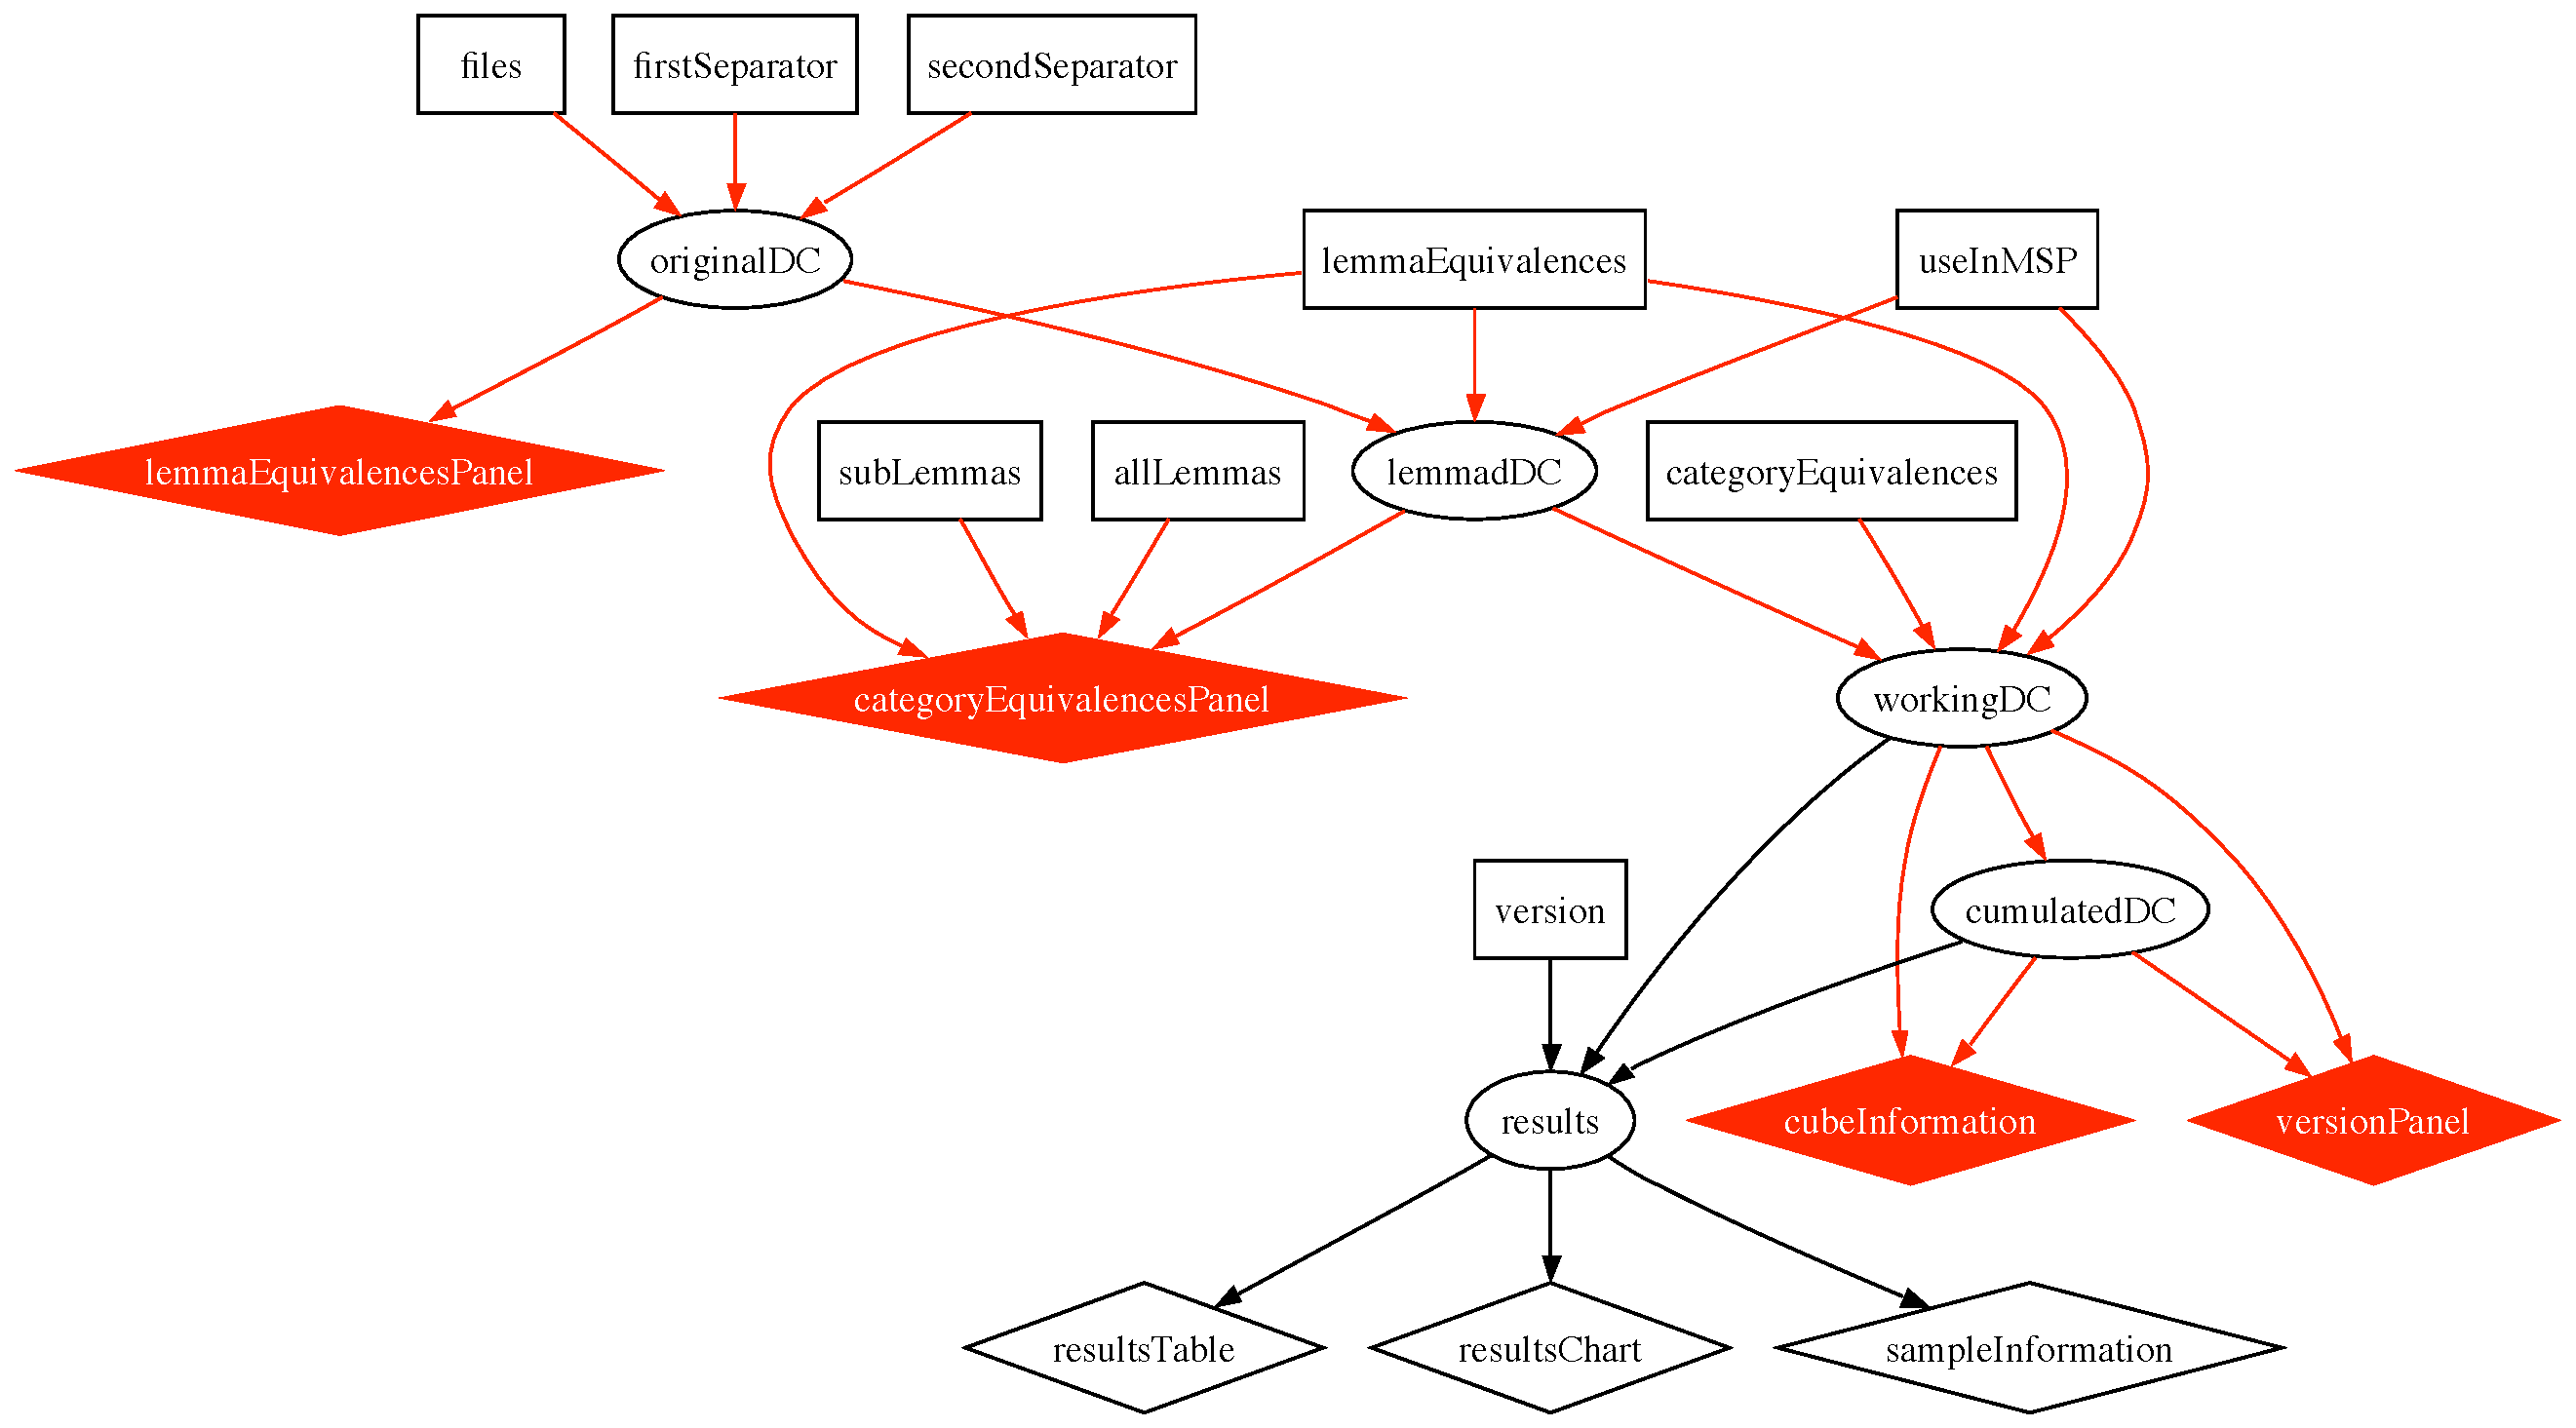
\includegraphics[scale=0.3]{dataflow}
	\caption{An overview of the cells and connections between the cells of MSPMeter.  \label{fig:cells}}
	\end{center}
\end{figure}


\subsection{Cells}
\begin{description}
\item[\texttt{files}] Contains an ordered list of spans. A \emph{span} is a set of files, together making up a logic unit the development of a child. For example, the speech of a child is recorded several times each month. All sessions recorded in one month are then bundled in a single span. 

\item[\texttt{firstSeparator}] Equals the value entered in the ``Token indicating lemma:''-field in the GUI. The characters entered in this field indicate the start of a lemma.

\item[\texttt{secondSeparator}] Equals the value entered in the ``Token between lemma and category:''-field in the GUI. The characters entered in this field indicate the separation between lemma and category. 

\item[\texttt{originalDC}] Is the data cube constructed by taking the files from the \texttt{files} cell and the characters from the \texttt{firstSeparator} and \texttt{secondSeparator}. In other words, this data cube contains the unprocessed data.

\item[\texttt{lemmaEquivalencesPanel}] Uses the \texttt{originalDC} to generate a default set of lemma equivalences (namely every lemma has its own equivalence class). 

\item[\texttt{lemmaEquivalences}] The result of the lemma equivalences panel: a set of lemma equivalences. 

\item[\texttt{useInMSP}] Corresponds to the ``Use in MSP''-checkbox in the GUI. If the cell's value is True, the lemma equivalences are used during the computation of MSP. Otherwise, the lemma equivalences are ignored (not sure why I did this).

\item[\texttt{lemmadDC}] The original data cube with lemma equivalences applied. If no lemma equivalences are applied, this equals the value of \texttt{originalDC}.

\item[\texttt{allLemmas}] Contains the set of all lemmas present in the original DC. It receives it information from the \texttt{lemmaEquivalencesPanel}. 

\item[\texttt{subLemmas}] Contains for each lemma the sublemmas. It receives it information from the \texttt{lemmaEquivalencesPanel}.

\item[\texttt{categoryEquivalencesPanel}] The panel in which the category equivalences are loaded and edited. 

\item[\texttt{categoryEquivalences}] Contains the category equivalence classes. 

\item[\texttt{workingDC}] Contains the data cube on which MSPMeter will work. Depending on the availability of lemma and category equivalences this data cube equals either the original data cube, the lemma'd data cube (if only lemma equivalences are specified) or the lemma'd data cube with category equivalences applied (if category equivalences, and possibly lemma equivalences, have been set).

\item[\texttt{cumulatedDC}] Contains the data cube in which cumulation has been applied across the span-dimension. 

\item[\texttt{cubeInformation}] This panel contains all kinds of information about the working data cube and the cumulated data cube: like the total number of lemmas, the sizes of the spans, etc, both for the working and cumulated data.

\item[\texttt{versionPanel}] In this panel the user specifies the sampling strategy and which version of MSP is calculated. Therefore, we need information about the number of lemmas in the spans, both in the working and cumulated data cube.

\item[\texttt{version}] Contains the parameters for the calculating of the MSP. 

\item[\texttt{results}] Contains the MSP values and the standard deviations. 

\item[\texttt{resultsTable}] The table displaying the MSP values and the standard deviations.

\item[\texttt{resultChart}] The chart displaying the MSP values and the standard deviations.

\item[\texttt{sampleInformation}] Displays the MSP value for each sample of each span.
\end{description}



\subsection{Flowing through the Grid}

Whenever the content of a cell changes (signaled to the grid by the cell itself), information starts flowing in the grid. When adding connections between cells, the grid also keeps track of the closure of the network. In the closure, a cell is connected to all cells that are influenced by a change in the first cell. For example, if cell A is connected to cell B and cell B is connected to cell C, cell A will be connected to both cell B and cell C in the closure. Indeed, if cell A changes value, this will flow to cell B. The change in cell B can possibly change the value of cell C. 

At the moment cell A signals a change, two possible scenarios unfold. If cell A is connected to a hot-flowing cell in the closure, all hot-flowing descendants of cell A are added to the \emph{hot queue}, scheduled to be recomputed as soon as possible. All cold-flowing descendants of cell A are added to the \emph{cold queue}, scheduled to be recomputed whenever the user instructs. Both queues are ordered, based on the structure of the grid. A cell is not recomputed before all its ancestors in the queue (cells linking to that cell in the closure) are have been recomputed. For example, suppose cell A is connected to cell B and cell C, and cells B and C are connected to cell D. All are hot-flowing. A change in cell A results in the addition of cells B, C and D to the hot queue. The order in which cells B and C are recomputed is unimportant. However, it is very important that cells B and C are recomputed before cell D is recomputed. Indeed, if we would recompute cell B, then recompute cell D and finish with recomputing cell C, cell D would not have the correct value because the recomputing of cell C can have important information for the recomputing of cell D. 

If a cell is not a predecessor of a hot-flowing cell, then a change in the cell is recorded, by the addition of the cell and its descendants in the cold queue. The change has no direct consequence on other cells or the GUI, because all recomputations are delayed until the user directs MSPMeter to compute.



\section{Sampling}

Several sampling algorithms have been implemented in MSPMeter. A sampling procedure has two \emph{scopes} either sampling occurs on the span-level or on the corpus-level. Sampling on the span-level implies that a number of samples are taken for each span. The MSP for each sample of the span is calculated and the MSP value for the span is the average value of the samples. Sampling on the corpus-level draws samples from the whole corpus, i.e.\ it is possible that some spans in a sample of the corpus are empty. All three sampling procedures work both for the span- and corpus-level. 

Secondly, the user has control over the \emph{number of samples}. Again there are two options. Either the user choose a sampling factor or a fixed number of samples. If the user enters a \emph{sampling factor}, denoted by $\sigma$, the sampling algorithm will automatically determine the number of samples, denoted $n$, for a span/corpus, denoted by $\mathcal{D}$, by applying the following formula: 
$$n = \lceil \frac{\sigma \times |\mathcal{D}|}{S} \rceil$$
where $S$ is the sample size. In other words, averaging over all sets of samples, each token will occur $\sigma$ times. 

All samplers view the initial data in the same way: the data is one long array of tokens. If a token occurs, for example, three times in the data, three (consecutive) spaces in the array are filled with this token. Let $\mathcal{D}$ be the dataset, then we denote by $A(\mathcal{D})$ the array of the dataset.

\subsection{Sampling Factor Sampler}

The user specifies a sample size $S$. This sampler will then generate samples that are \emph{on average} of size $S$. It generates a sample by running over $A(\mathcal{D})$ and selecting a token with probability:
$$\frac{S}{|A(\mathcal{D})|} \enspace.$$

Clearly, it is not guaranteed that a sample is of size $S$, however, on average it will be.



\subsection{Improved Sampling Factor Sampler}

An improvement on the previous sampler, makes sure that each sample is of size $S$. Let $i$ be the number of already selected tokens and let $m$ the number of tokens already visited in the array. The improved sampling factor sampler runs over $A(\mathcal{D})$ and selects a token with probability:
$$\frac{S-i}{N-m} \enspace.$$ 

Clearly, if the sample already contains $S$ tokens, the probability drops to zero, i.e.\ no more tokens are selected. On the other hand, if the sampler reaches the end of the array, and the sample is not yet full, the probability will go up, as the difference between $S-i$ and $N-m$ diminishes.


\subsection{Fixed Size Sampler}

Analogous to the Improved Sampling Factor Sampler, the Fixed Size Sampler needs the user to specify the size of the samples. Unlike the previous sampler, this sampler starts picking tokens from $A(\mathcal{D})$ until the sample is full. Once a token is picked from the dataset, it is removed from the dataset, i.e.\ if a token occurs four times in the dataset, it cannot occur more than four times in any sample. In other words, this sampler takes an arbitrary combination of size $S$ of the data. 






\section{Input/Output}

MSPMeter operates on several different types of files. 



\subsection{Input files}

Files that can be used as input to MSPMeter, are \emph{frequency files}. A frequency file is basically a text file obliging to a certain syntax. A line in a frequency file consists of two parts: a \emph{count} and \emph{token-data}. Both parts are separated by a whitespace. The token-data contains two important pieces of information: a lemma and a category, although the category may not be present. In most cases the pipe ($|$) indicates the start of the lemma. The end of the lemma is either a newline or a character indicating the start of the category. 

Lines that are not in accord to this form are discarded.


\subsection{Project files}

A project file is an XML-formatted file, which stores the input of the user in MSPMeter, i.e.\ which files are the input, which version of MSP, which lemma equivalences, etc. The structure of the project file is described in the file \texttt{project.xsd}, a XML Schema file defining the valid files. The classes \texttt{ProjectReader} (based on a SAX parser) and \texttt{ProjectWriter} are responsible for reading and writing the project files.


\subsection{Result files}

The MSP values of a set of spans can be saved in different formats. Concretely:
\begin{itemize}
\item \emph{CSV} (Comma-Separated Values): exports a file containing three fields (span name, MSP and standard deviation of MSP) separated by commas. 

\item \emph{Tab-delimited}: exports a file containing three fields (span name, MSP and standard deviation of MSP) separated by tabs. 

\item \emph{Excel}: exports an Excel sheet with three columns (span name, MSP and standard deviation of MSP). 

\item \emph{XML}: exports a XML file with three fields (span name, MSP and standard deviation of MSP).
\end{itemize}



\end{document}
